% !TeX root = RJwrapper.tex
\title{Geographic visualization and analysis in R with tigris}
\author{by Kyle Walker, Bob Rudis}

\maketitle

\abstract{%
The TIGER/Line shapefiles from the United States Census Bureau are
commonly used for the mapping and analysis of US demographic trends. The
\texttt{tigris} package provides a uniform interface for R users to
download and work with these shapefiles. Functions in \texttt{tigris}
allow R users to request Census geographic datasets using familiar
geographic identifiers and return those datasets as Spatial DataFrames.
Once downloaded, \texttt{tigris} helps R users flexibly combine
geographic datasets and join them to tabular data. In turn,
\texttt{tigris} helps facilitate both the visualization of and analysis
spatial data in R. This article provides an overview of such geospatial
workflows in R, and illustrates how the tigris package can assist with
such workflows by providing programmatic access to spatial data.
}

\subsection{Introduction}\label{introduction}

Analysis and visualization of geographic data are often core components
of the analytical workflow for researchers and data scientists; as such,
access to open and reliable geographic datasets are of paramount
importance. The United States Census Bureau provides access to such data
in the form of its TIGER/Line shapefile products. The files are extracts
from the Census Bureau's Master Address File/Topologically Integrated
Geographic Encoding and Referencing (TIGER) database, which in turn are
released to the public as shapefiles, a common format for encoding
geographic data as vectors (e.g.~points, lines, and polygons). Available
TIGER/Line shapefiles include all of the Census Bureau's areal
enumeration units, such as states, counties, Census tracts, and Census
blocks; transportation data such as roads and railways; and both linear
and areal hydrography. The TIGER/Line files are updated annually, and
include columns that allow them to be joined with other tabular data,
including demographic data products released by the Census Bureau
\citep{Census}.

The \CRANpkg{tigris} package aims to simplify the process of working
with these datasets for R users. With functions in tigris, R users can
specify the data type and geography for which they would like to obtain
geographic data, and return the corresponding TIGER/Line data as an R
object of class \texttt{Spatial*DataFrame} as read in by the
\texttt{rgdal} package. This article provides an overview of the
\texttt{tigris} package, and gives examples that show how it can
contribute to common geographic visualization and spatial analysis
workflows in R. The first section explains the core functionality of the
package; the second section discusses how R users can create both static
and interactive visualizations with data from the package, leveraging
functionality in R packages like \CRANpkg{ggplot2}, \CRANPkg{rgeos}, and
\CRANPkg{leaflet}; and the final section shows how tigris can integrate
with spatial statistics packages like \CRANPkg{GWModel} to facilitate
geospatial analyses.

\subsection{Geographic data and Census visualization in
R}\label{geographic-data-and-census-visualization-in-r}

To cover:

\begin{itemize}
\tightlist
\item
  Overview of the TIGER/Line shapefiles
\item
  Objects of class \texttt{Spatial} in R and the \texttt{rgdal} package
\item
  Other packages, including:

  \begin{itemize}
  \tightlist
  \item
    \texttt{USCensus2010}
  \item
    \texttt{acs}
  \item
    \texttt{choroplethr}
  \end{itemize}
\item
  Space \texttt{tigris} occupies - uniform interface for downloading and
  delimiting all TIGER/Line and cartographic boundary shapefiles
\end{itemize}

\subsection{Core functionality}\label{core-functionality}

The core functionality in tigris involves the usage of a series of
functions, each corresponding to a single Census Bureau geography of
interest, to access geographic data from the US Census Bureau. tigris
grants access to both the core TIGER/Line shapefiles as well as the
Census Bureau's Cartographic Boundary Files. Cartographic Boundary
Files, following the Census Bureau (2015), ``are simplified
representations of selected geographic areas from the Census Bureau's
MAF/TIGER geographic database'' \citep{Census2015}. However, these files
are also clipped to the shoreline of the United States, which can
introduce additional detail for coastal features.

To download geographic data using tigris, the R user calls the function
corresponding to the desired geography. For example, to obtain a
\texttt{SpatialPolygonsDataFrame} of US states from the TIGER/Line
dataset, the user calls the \texttt{states} function in tigris, which
can then be plotted with the \texttt{plot} function from the
\CRANPkg{sp} package:

\begin{Schunk}
\begin{Sinput}
library(tigris)
library(sp)

us_states <- states()

plot(us_states)
\end{Sinput}

\includegraphics{walker-rudis_files/figure-latex/unnamed-chunk-1-1} \end{Schunk}

The \texttt{states} function call instructs tigris to fetch a TIGER/Line
shapefile from the US Census Bureau that represents the boundaries of
the 50 US states, the District of Columbia, and US territories. tigris
then uses the \CRANPkg{rgdal} package to load the data into the user's R
session as an object of class \texttt{Spatial\ DataFrame}. Many
functions in tigris have a parameter, \texttt{cb}, that if set to
\texttt{TRUE} will direct tigris to load a cartographic boundary file
instead. Cartographic boundary files default to a simplified resolution
of 1:500,000; in some cases, as with states, resolutions of 1:5 million
and 1:20 million are example. For example, an R user could specify the
following modifications to the \texttt{states} function, and retrieve a
simplified dataset.

\begin{Schunk}
\begin{Sinput}
us_states_20m <- states(cb = TRUE, resolution = '20m')
\end{Sinput}
\begin{Soutput}
#> Warning in readOGR(dsn = cache_dir, layer = shape, encoding = "UTF-8",
#> verbose = FALSE, : Z-dimension discarded
\end{Soutput}
\begin{Sinput}
ri <- us_states[us_states$NAME == 'Rhode Island', ]
ri_20m <- us_states_20m[us_states_20m$NAME == 'Rhode Island', ]

plot(ri)
plot(ri_20m, border = 'red', add = TRUE)
\end{Sinput}

\includegraphics{walker-rudis_files/figure-latex/unnamed-chunk-2-1} \end{Schunk}

The plot illustrates some of the differences between the TIGER/Line
shapefiles and the cartographic boundary files, in this instance for the
state of Rhode Island. TIGER/Line files include water area, whereas the
cartographic boundary files do not; however, in interior areas, they are
not nearly as detailed.

In many instances, Census geographic data are only available at
sub-national levels, or the R user might want to specify how to subset
the data geographically \emph{a priori} by state and optionally county.
Census geographic data are referenced, however, by their Federal
Information Processing Standard (FIPS) codes, which are codes that
uniquely identify geographic entities in the Census database. When
applicable, tigris uses smart state and county lookup to simplify this
process for R users, allowing users to subset data based on the name or
postal code of the desired state, or name of the county, rather than
their FIPS codes.

\begin{Schunk}
\begin{Sinput}
kw_roads <- roads('HI', 'Kalawao')
\end{Sinput}
\begin{Soutput}
#> Using FIPS code '15' for state 'HI'
#> Using FIPS code '005' for 'Kalawao County'
\end{Soutput}
\begin{Sinput}
plot(kw_roads)
\end{Sinput}

\includegraphics{walker-rudis_files/figure-latex/unnamed-chunk-3-1} \end{Schunk}

When tigris downloads Census shapefiles to the R user's computer, it
uses the \CRANPkg{rappdirs} package to cache the downloads for future
access. In turn, once the R user has downloaded the Census geographic
data, tigris will know where to look for it and will not need to
re-download.

Some Census shapefiles, like roads, are only available by county;
however, an R user may want a roads dataset that represents multiple
counties. tigris has built-in functionality to handle these
circumstances. Data loaded into R by tigris have a special attribute,
\texttt{tigris\_type}, that identifies the type of geographic data
represented by the object. In turn, objects of the same
\texttt{tigris\_type} can be combined using the function
\texttt{rbind\_tigris}, which takes multiple tigris objects (or
optionally a list) and combines them into a single object.

\begin{Schunk}
\begin{Sinput}
tigris_type(kw_roads)
\end{Sinput}
\begin{Soutput}
#> [1] "road"
\end{Soutput}
\end{Schunk}

\begin{Schunk}
\begin{Sinput}
maui_roads <- roads('HI', 'Maui')
\end{Sinput}
\begin{Soutput}
#> Using FIPS code '15' for state 'HI'
#> Using FIPS code '009' for 'Maui County'
\end{Soutput}
\begin{Sinput}
maui_kw_roads <- rbind_tigris(kw_roads, maui_roads)

plot(maui_kw_roads)
\end{Sinput}

\includegraphics{walker-rudis_files/figure-latex/unnamed-chunk-5-1} \end{Schunk}

The Census Bureau releases updated TIGER/Line shapefiles every year, and
these yearly updates are available to tigris users. tigris defaults to
the 2014 shapefiles, which at the time of this writing is the most
recent year available for the cartographic boundary files. However,
tigris users can supply a different year to a tigris function as a named
argument to obtain data for a different year; for example,
\texttt{year\ =\ 2015} in the function call will fetch the most recent
TIGER/Line shapefiles from 2015. Additionally, R users can set this as a
global option in their R session by entering the command
\texttt{options(tigris\_year\ =\ 2015)}.

\subsection{\texorpdfstring{Visualization with
\texttt{tigris}}{Visualization with tigris}}\label{visualization-with-tigris}

A core component of geospatial analysis in R is mapping and
visualization, and tigris assists with this by providing programmatic
access to quality US Census geographic datasets for R users. On a basic
level, R users can quickly visualize tigris datasets with the
\texttt{plot} function available in \CRANPkg{sp}, as evidenced in the
examples above. tigris objects also work well with the popular
\CRANPkg{ggplot2} package for visualization in R. The example below uses
ggplot2 to visualize state legislative districts in Vermont from tigris:

\begin{Schunk}
\begin{Sinput}
library(tigris)
library(ggplot2)
library(ggthemes)

vt <- state_legislative_districts('Vermont', house = 'upper', cb = TRUE)
\end{Sinput}
\begin{Soutput}
#> Using FIPS code '50' for state 'Vermont'
\end{Soutput}
\begin{Sinput}
vt_map <- fortify(vt)
\end{Sinput}
\begin{Soutput}
#> Regions defined for each Polygons
\end{Soutput}
\begin{Sinput}
ggplot() + 
  geom_map(data = vt_map, map = vt_map, 
           aes(x = long, y = lat, map_id = id), 
           color = "navy", fill = "lightgrey", 
           size = 0.25) + 
  coord_map() + 
  theme_map()
\end{Sinput}

\includegraphics{walker-rudis_files/figure-latex/unnamed-chunk-6-1} \end{Schunk}

Commonly, geographic visualization will involve more that just plotting
the outlines of the data, however. Instead, practitioners will want to
use mapping to show the geographic distribution of some attribute of
interest, which may be derived from some analysis in an R data frame. To
facilitate this process, tigris includes a function, \texttt{geo\_join},
to ease the sometimes-messy process of merging tabular data to spatial
data frames. Such joined data can then be used for statistical mapping,
such as with a choropleth map that shows variation in an attribute by
the shading of polygons.

In turn, data functions in tigris along with \texttt{geo\_join} can be
used in visualization workflows alongside spatial data management and
mapping packages in R. The following example uses \texttt{geo\_join} to
merge spatial data from tigris to demographic data from the
\CRANPkg{acs} package, and then creates a static map from the data with
the \CRANPkg{tmap} package for thematic mapping.

The R user first loads the three main libraries, in addition to
\CRANPkg{stringr} and rgdal for data processing. The user specifies the
names of counties for which to fetch Census tract spatial data, and
passes this to the \texttt{tracts} function to create an object of class
\texttt{SpatialPolygonsDataFrame} representing Census tracts in the
Dallas-Fort Worth, Texas metropolitan area.

\begin{Schunk}
\begin{Sinput}
library(tigris)
library(acs)
library(stringr)
library(tmap)
library(rgdal)

dfw_counties <- c('Dallas', 'Tarrant', 'Denton', 'Rockwall', 'Collin ', 
                  'Wise', 'Parker', 'Ellis', 'Kaufman', 'Hunt', 'Delta', 'Johnson')

dfw_tracts <- tracts('Texas', county = dfw_counties, cb = TRUE)
\end{Sinput}
\end{Schunk}

The next step involves fetching data from the US Census Bureau's data
API using the acs package. However, counties in the acs package are not
referenced by name, but rather by numeric FIPS codes. When loaded,
tigris also loads a data frame named \texttt{fips\_codes} that provides
a reference between the names of states and counties, and their
corresponding FIPS codes; this information in turn can be leveraged in a
function to convert the vector of county names to a vector of numeric
FIPS codes, and used to get demographic data, in this instance on median
household income, from the Census Bureau. The R user then merges the
demographic data to the shape data using tigris's \texttt{geo\_join}
function.

\begin{Schunk}
\begin{Sinput}
to_fips <- function(state, county_name) {
  with_county <- paste(county_name, 'County')
  sub1 <- fips_codes[fips_codes\$county == with_county & fips_codes\$state == state, ]
  return(as.numeric(sub1\$county_code))
    
}

dfw_fips <- sapply(dfw_counties, function(x) to_fips('TX', x))

income_data <- acs.fetch(endyear = 2012, 
                         geography = geo.make(state = "TX", 
                                              county = dfw_fips, 
                                              tract = "*"), 
                         variable = "B19013_001")

income_df <- data.frame(paste0(as.character(income_data@geography\$state), 
                               str_pad(as.character(income_data@geography\$county), 3, 'left', '0'), 
                               str_pad(as.character(income_data@geography\$tract), 5, 'left', '0')), 
                        income_data@estimate)

colnames(income_df) <- c("GEOID", "hhincome")

dfw_merged <- geo_join(dfw_tracts, income_df, "GEOID", "GEOID")
\end{Sinput}
\end{Schunk}

The data are now ready for visualization. To provide spatial reference
to the Census tracts on the map, major roads can be obtained with the
\texttt{primary\_roads} function in tigris, and added to the map as
well. The R user then projects the spatial data to an appropriate
projected coordinate system - in this case Universal Transverse Mercator
Zone 14N - and maps the data with functions in the tmap package.

\begin{Schunk}
\begin{Sinput}
rds <- primary_roads()

to_utm14n <- function(x) {
  return(spTransform(x, CRS('+init=epsg:26914')))
} 

tm_shape(to_utm14n(dfw_merged)) + 
  tm_fill('hhincome', style = 'quantile', n = 7, palette = 'Greens', title = '') + 
tm_shape(rds) + 
  tm_lines(col = 'darkgrey') + 
tm_layout(bg.color = 'ivory', title = 'Median household income by Census tract, Dallas-Fort Worth', 
          legend.position = c('right', 'bottom'), title.bg.color = 'ivory', legend.text.size = 1, 
          legend.width = 0.2, legend.frame = TRUE) + 
tm_credits('Data source: 2008-2012 American Community Survey', 
           position = c('left', 'bottom'))
\end{Sinput}
\end{Schunk}

\begin{figure}[htbp]
  \centering
  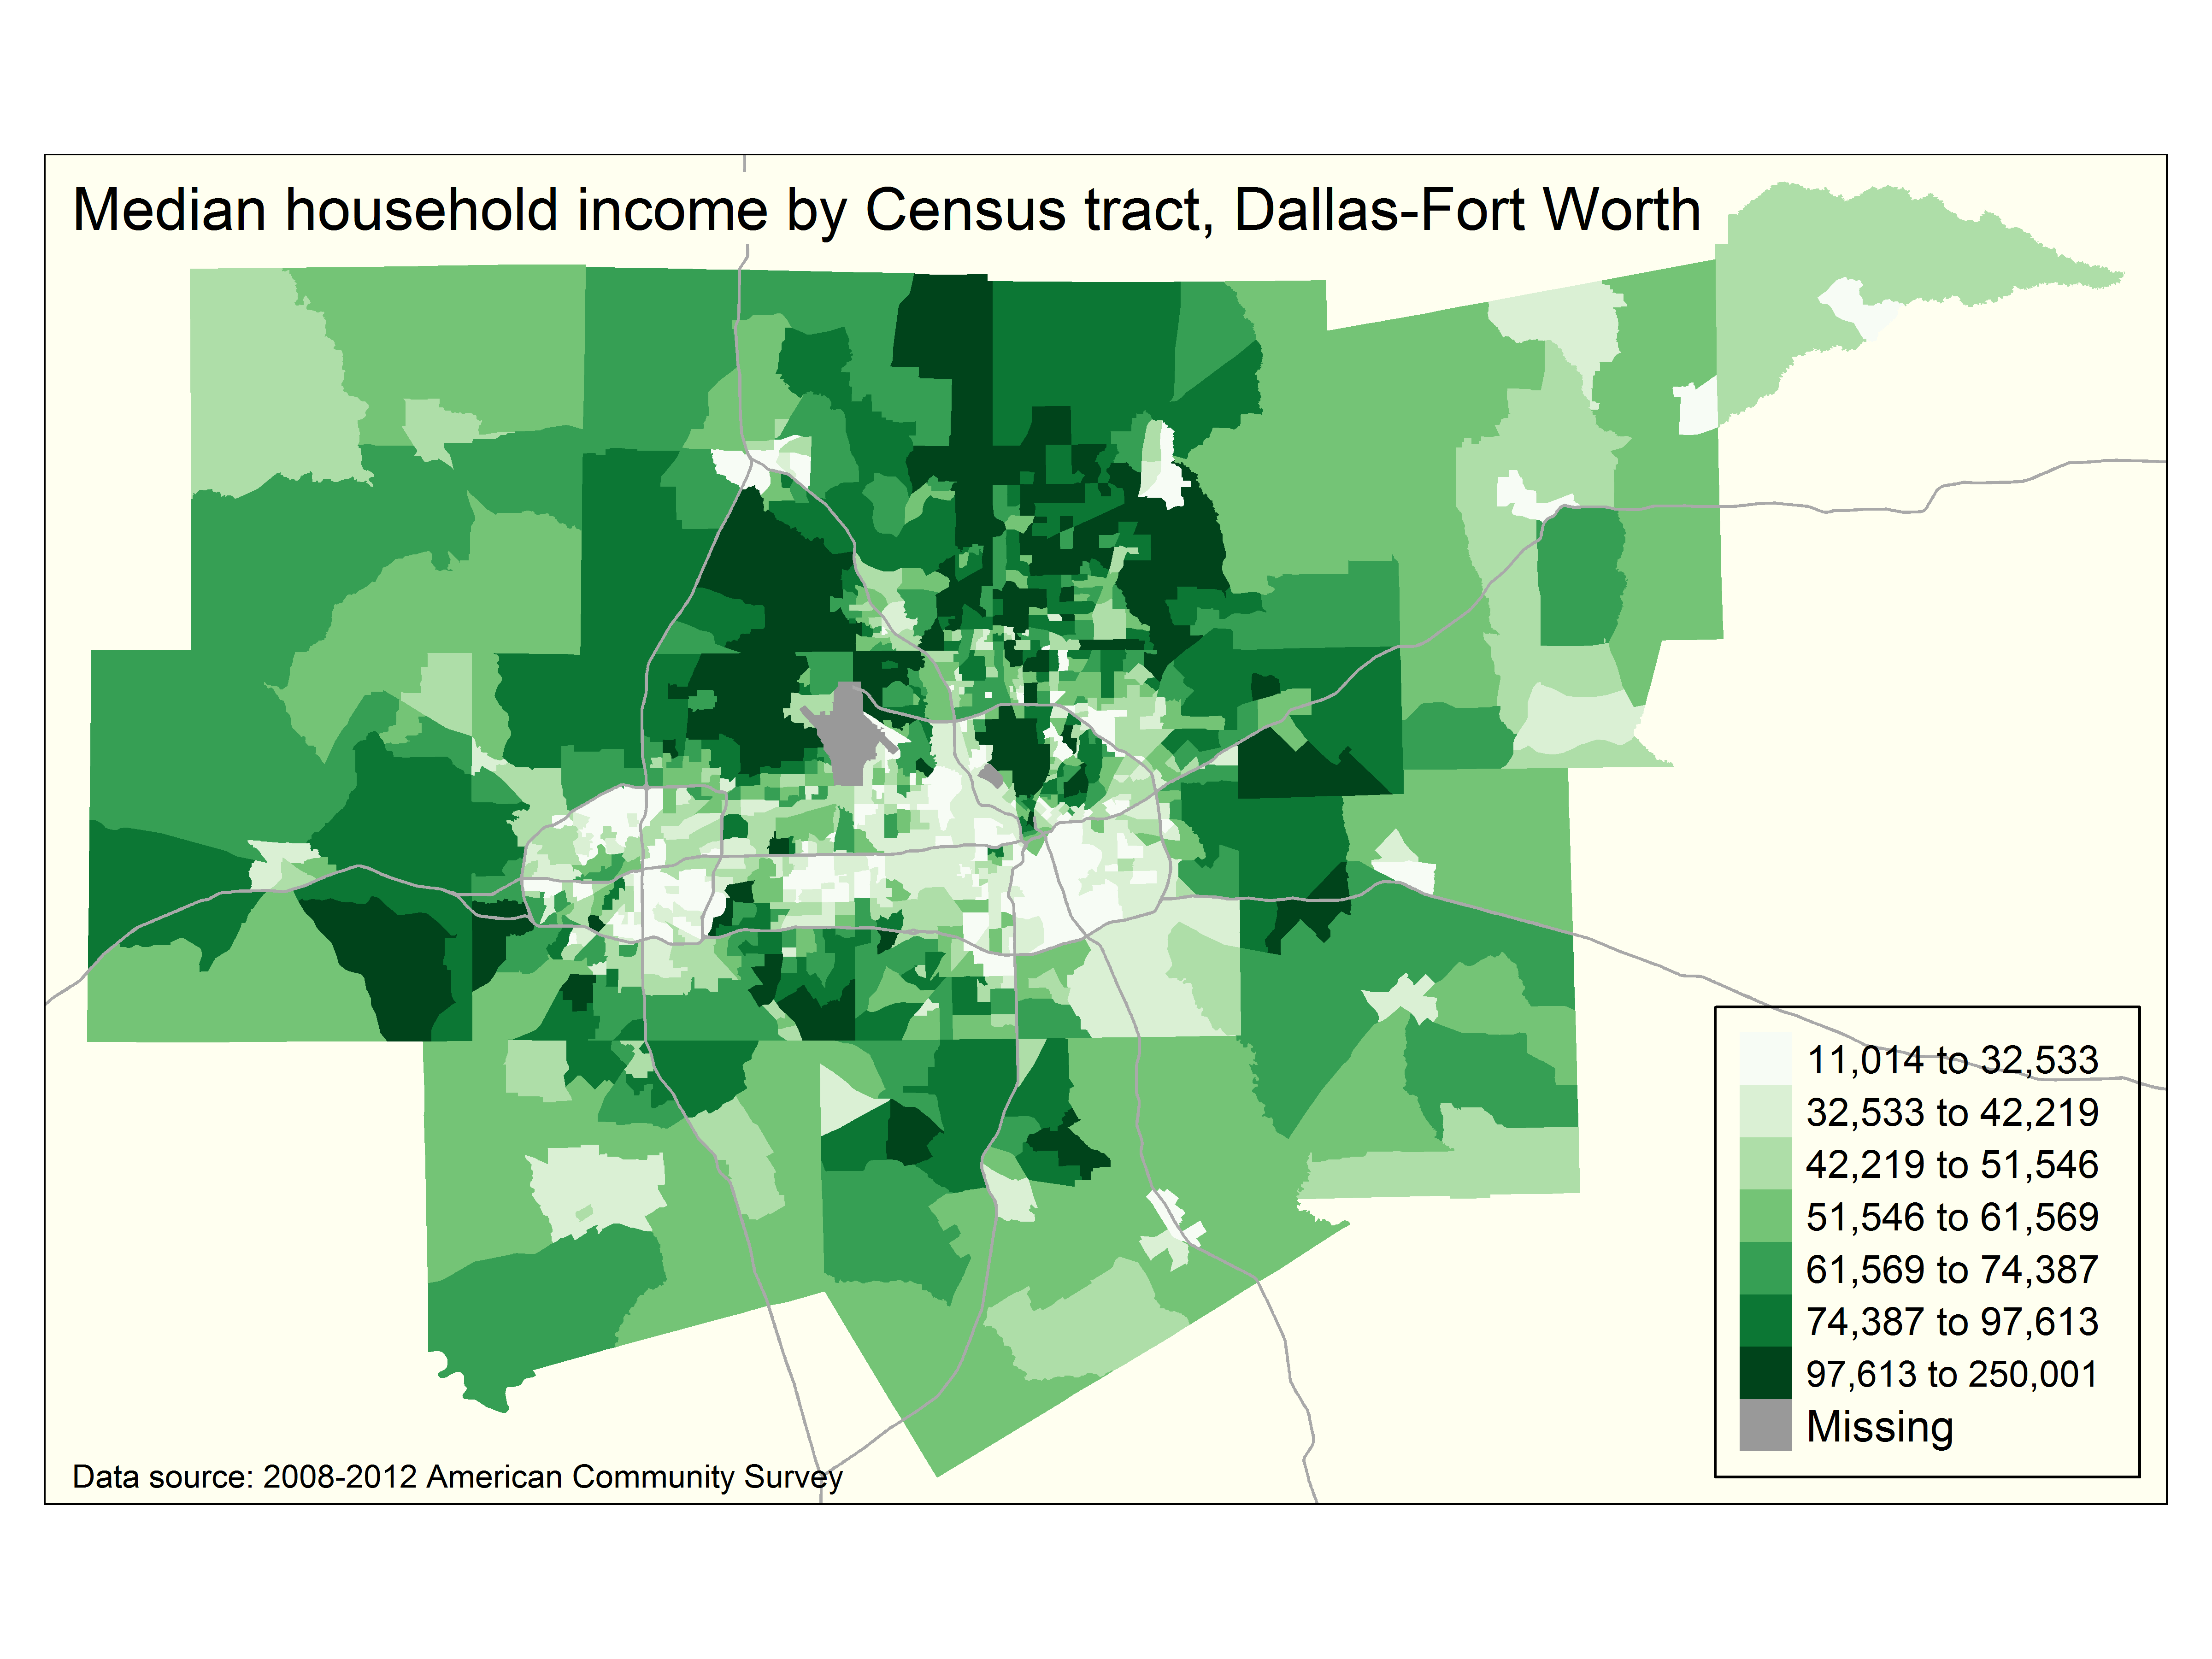
\includegraphics[width=\textwidth]{income_map}
  \caption{Map of median household income by Census tract in the Dallas-Fort Worth, Texas metropolitan area.}
  \label{figure:income_map}
\end{figure}

The resultant map is comparable to cartographic output from a desktop
geographic information system, and can be produced entirely within R
without having to seek out and download data externally.

\subsection{\texorpdfstring{Spatial analysis with
\texttt{tigris}}{Spatial analysis with tigris}}\label{spatial-analysis-with-tigris}

In addition to visualization, tigris works well within common spatial
analysis workflows in R. Geospatial analyses in R span a wide variety of
packages, but are arguably associated most commonly with the
\CRANPkg{rgeos} package, which is an R interface to the C Geometry
Engine - Open Source. The rgeos package includes functions that in many
cases mirror the analytical capabilities of geographic information
systems software.

Data from tigris alongside analytic functions from rgeos equips R users
to quickly answer a host of common geographic questions using Census
data. The previous example showed how to visualize a quantitative
attribute from the American Community Survey using geographic data from
tigris, and added a second tigris layer, primary roads, to provide
reference. Spatial analysis functions from rgeos can explicitly consider
how different tigris layers relate to one another spatially, which in
turn can contribute to broader spatial analysis workflows.

Consider the following hypothetical example: an analyst wishes to
identify the Census block groups within 500 meters of the Red River in
Fargo, North Dakota. Functions in tigris combined with rgdal and rgeos
make this process straightforward. To begin, the analyst identifies
which datasets are needed to answer this question. Block groups are
available by state and optionally by county, and water features are
available by county within states; the \texttt{block\_groups} and
\texttt{linear\_water} functions can be called to fetch the requisite
data for Cass County, ND. Beyond this, the analyst will need to call the
\texttt{places} function to get outlines of Census-designated places,
which includes city boundaries; the outline of Fargo can be extracted
from here. Each function is wrapped in the \texttt{to\_utm14n} function
used earlier to transform the data for North Dakota into an appropriate
projected coordinate system. The analyst then subsets the data to
retrieve a \texttt{SpatialLinesDataFrame} that represents the Red River
from the original \texttt{water} dataset, and a
\texttt{SpatialPolygonsDataFrame} with one polygon representing the
shape of Fargo.

\begin{Schunk}
\begin{Sinput}
library(tigris)
library(rgeos)
library(rgdal)

to_utm14n <- function(x) {
  return(spTransform(x, CRS('+init=epsg:26914')))
} 
 
water <- to_utm14n(linear_water('ND', 'Cass'))

bgs <- to_utm14n(block_groups('ND', 'Cass'))

pl <- to_utm14n(places('ND'))

red_river <- gLineMerge(water[grep('Red Riv', water\$FULLNAME), ]) 

fargo <- pl[pl\$NAME == 'Fargo', ]
\end{Sinput}
\end{Schunk}

From here, the analyst can use spatial analysis functions available
within rgeos to retrieve the desired block groups. First, the analyst
calls \texttt{gWithin} to find the block groups that are located within
the city of Fargo, returning a new \texttt{SpatialPolygonsDataFrame}
named \texttt{fargo\_bgs}. Next, the \texttt{gDistance} function is used
to generate a new column in \texttt{fargo\_bgs} that represents the
distance from each block group to the Red River in meters, which is the
unit of measurement of the dataset's projected coordinate system.
Finally, the analyst can subset \texttt{fargo\_bgs} to identify those
block groups with a distance value less than 500 meters.

\begin{Schunk}
\begin{Sinput}
fargo_bgs <- bgs[as.vector(gWithin(bgs, fargo, byid = TRUE)), ]

fargo_bgs\$distance <- as.vector(gDistance(fargo_bgs, red_river, byid = TRUE))

within_500m <- fargo_bgs[fargo_bgs\$distance < 500, ]
\end{Sinput}
\end{Schunk}

These results can then be visualized using the \CRANPkg{ggmap} package:

\begin{Schunk}
\begin{Sinput}
library(ggmap)

fargo_xy <- spTransform(within_500m, CRS("+proj=longlat +datum=WGS84"))

data <- fortify(fargo_xy)

ggmap(get_map(location = 'Fargo', zoom = 12, source = 'stamen', maptype = 'toner-lite')) + 
  geom_polygon(data = data, aes(x = long, y = lat, group = group), 
               alpha = 0.5, fill = 'blue', color = 'black')
\end{Sinput}
\end{Schunk}

\begin{figure}[htbp]
  \centering
  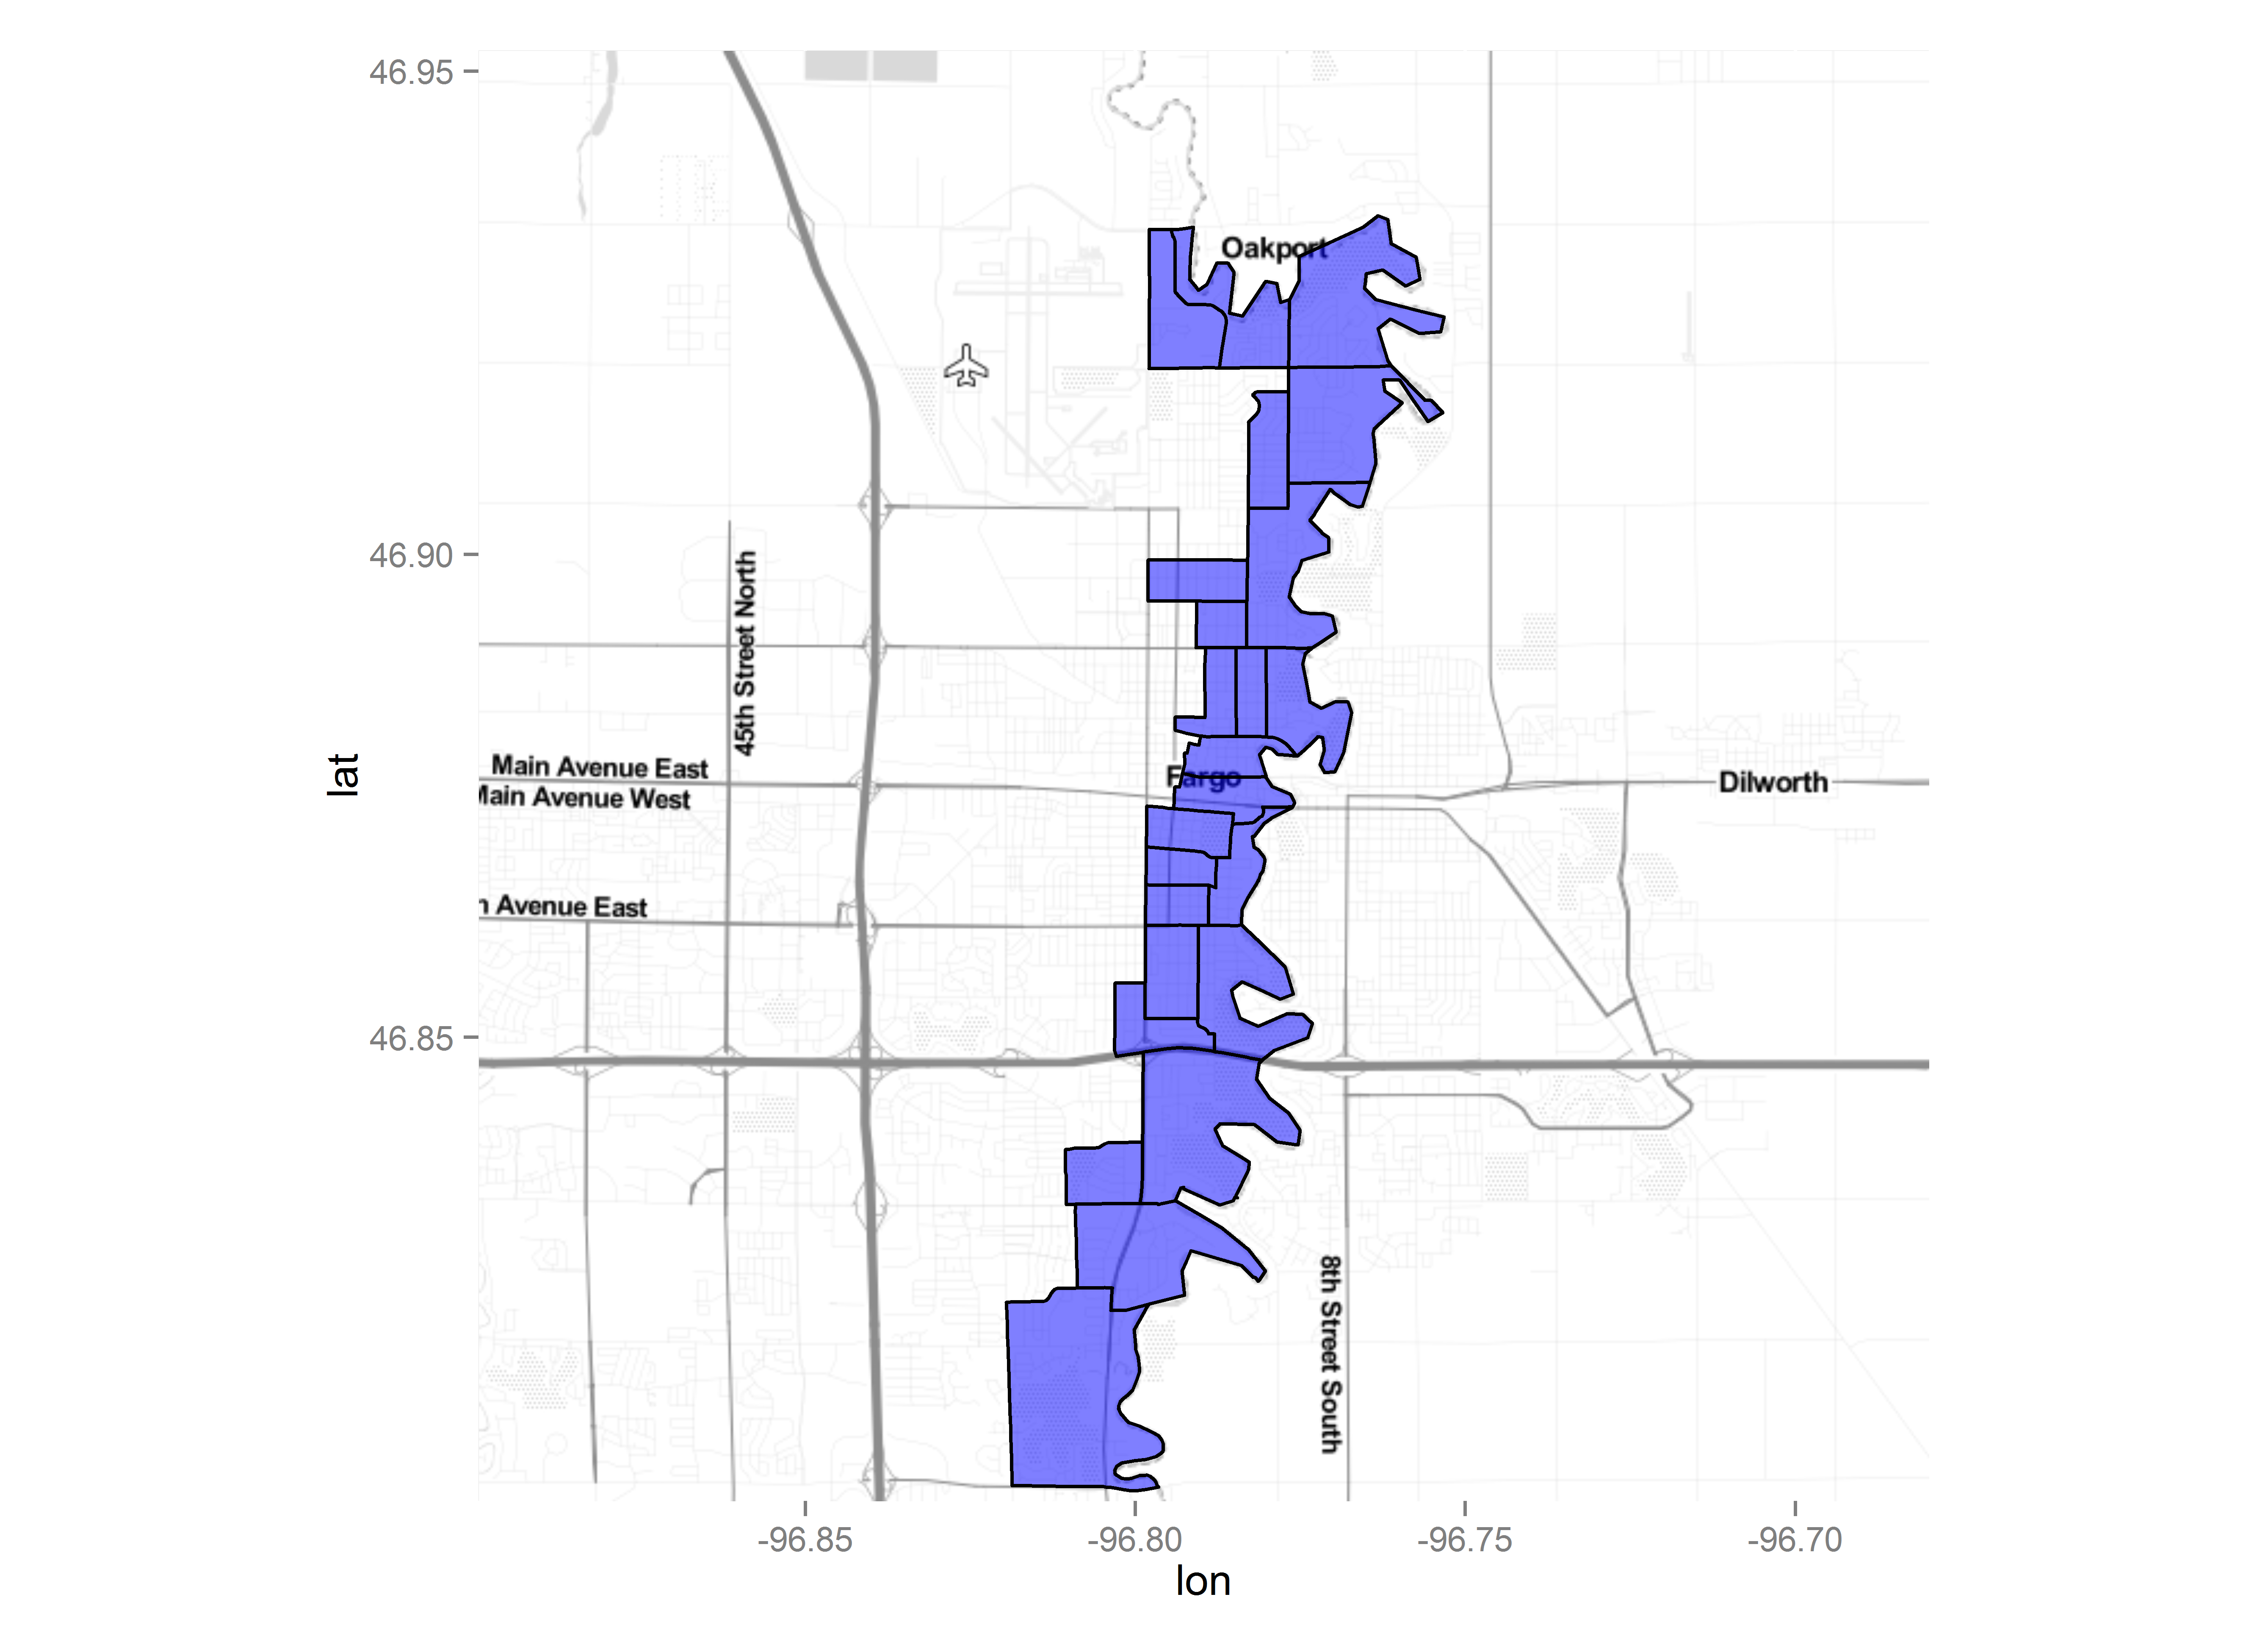
\includegraphics[width=\textwidth]{fargo_map}
  \caption{Block groups in Fargo, North Dakota within 500m of the Red River.}
  \label{figure:fargo_map}
\end{figure}

In this example, the entire process of data retrieval and subsetting
through spatial analysis, which commonly requires multiple steps in a
traditional GIS environment, is reduced to a few lines of R code.

\subsection{Putting it all together: mapping data from the US Internal
Revenue
Service}\label{putting-it-all-together-mapping-data-from-the-us-internal-revenue-service}

To this point, this paper has employed simplified examples to
demonstrate the functionality of tigris; the following scenario combines
these examples into an applied analytic and visualization workflow. This
example presumes that an R user would like to produce a series of
interactive maps for major US metropolitan areas using aggregated
taxation data from the United States Internal Revenue Service (IRS),
which are made available at the zip code level. Zip codes, however, are
not physical areas but rather designations given by the United States
Postal Service (USPS) to guide mail routes. The US Census Bureau
provides approximations of zip code geography, called Zip Code
Tabulation Areas (ZCTAs). ZCTAs are geographies built from Census blocks
that comprise those blocks in which a plurality (check this) of street
addresses have a given zip code. ZCTAs are available in tigris from the
\texttt{zctas} function.

Additionally, ZCTAs do not have a clear correspondence between their
boundaries and those of other Census units; in turn, ZCTA boundaries
will commonly cross those of metropolitan areas, which are county-based.
However, tigris provides programmatic access to metropolitan area
boundaries as well, which in turn can be used to identify intersecting
ZCTAs through spatial overlay with the \CRANPkg{rgeos} package. The
resultant spatial data can then be merged to data from the IRS and
visualized.

Such a workflow could resemble the following. An analyst reads in raw
data from the IRS website as an R data frame, and uses the
\CRANPkg{dplyr} package to subset the data frame and identify the
average total income reported to the IRS by zip code, assigning it to
the variable \texttt{df}.

\begin{Schunk}
\begin{Sinput}
library(dplyr)
library(stringr)
library(readr)

# Read in the IRS data
zip_data <- 'https://www.irs.gov/pub/irs-soi/13zpallnoagi.csv'

df <- read_csv(zip_data) %>%
  mutate(zip_str = str_pad(as.character(ZIPCODE), width = 5, side = 'left', pad = '0'), 
         incpr = A02650 / N02650) %>%
  select(zip_str, incpr)
\end{Sinput}
\end{Schunk}

The analyst then defines a function that will leverage tigris to read in
Census ZCTA and metropolitan area datasets as objects of class
\texttt{SpatialPolygonsDataFrame}, and return the ZCTAs that intersect a
given metropolitan area as defined by the analyst.

\begin{Schunk}
\begin{Sinput}
library(tigris)
library(rgeos)

# Write function to get ZCTAs for a given metro
get_zips <- function(metro_name) {
  
  zips <- zctas(cb = TRUE)
  
  metros <- core_based_statistical_areas(cb = TRUE)
  
  # Subset for specific metro area (be careful with duplicate cities like "Washington")
  my_metro <- metros[grepl(sprintf("\^%s", metro_name), metros\$NAME, ignore.case = TRUE), ]
  
  # Find all ZCTAs that intersect the metro boundary
  my_zips <- zips[as.vector(gIntersects(zips, my_metro, byid = TRUE)), ]
  
  # Return those ZCTAs
  return(my_zips)

}
\end{Sinput}
\end{Schunk}

Next, the analyst writes a second function to create an interactive map
of the ZCTAs with the \CRANPkg{leaflet} package, which converts objects
of class \texttt{Spatial*DataFrame} to interactive, web-based maps using
the \CRANPkg{htmlwidgets} package.

\begin{Schunk}
\begin{Sinput}
library(leaflet)

# Function to map the IRS data
map_zips <- function(data, palette = "PuRd") {
  
  data_merged <- geo_join(data, df, "ZCTA5CE10", "zip_str")

  pal <- colorQuantile(palette, NULL, n = 7, na.color = '#DBDBDB')
  
  label <- paste0("Zip Code ", data_merged\$ZCTA5CE10, ": \$", 
                  as.character(round(1000 * data_merged\$incpr, 2)))
  
  leaflet() %>%
    addProviderTiles("CartoDB.DarkMatter") %>%
    addPolygons(data = data_merged, 
                fillColor = ~pal(data_merged\$incpr), 
                fillOpacity = 0.7, 
                weight = 0.2, 
                smoothFactor = 0.2, 
                label = label) %>%
    addLegend(pal = pal, 
              values = round(1000 * data_merged\$incpr, 2), 
              position = "bottomright", 
              title = "Average reported income to IRS")

}
\end{Sinput}
\end{Schunk}

The analyst can then call the functions to create custom IRS taxation
maps by metro area as desired. For example:

\begin{Schunk}
\begin{Sinput}
get_zips('Nashville') %>% map_zips()
\end{Sinput}
\end{Schunk}

\begin{figure}[htbp]
  \centering
  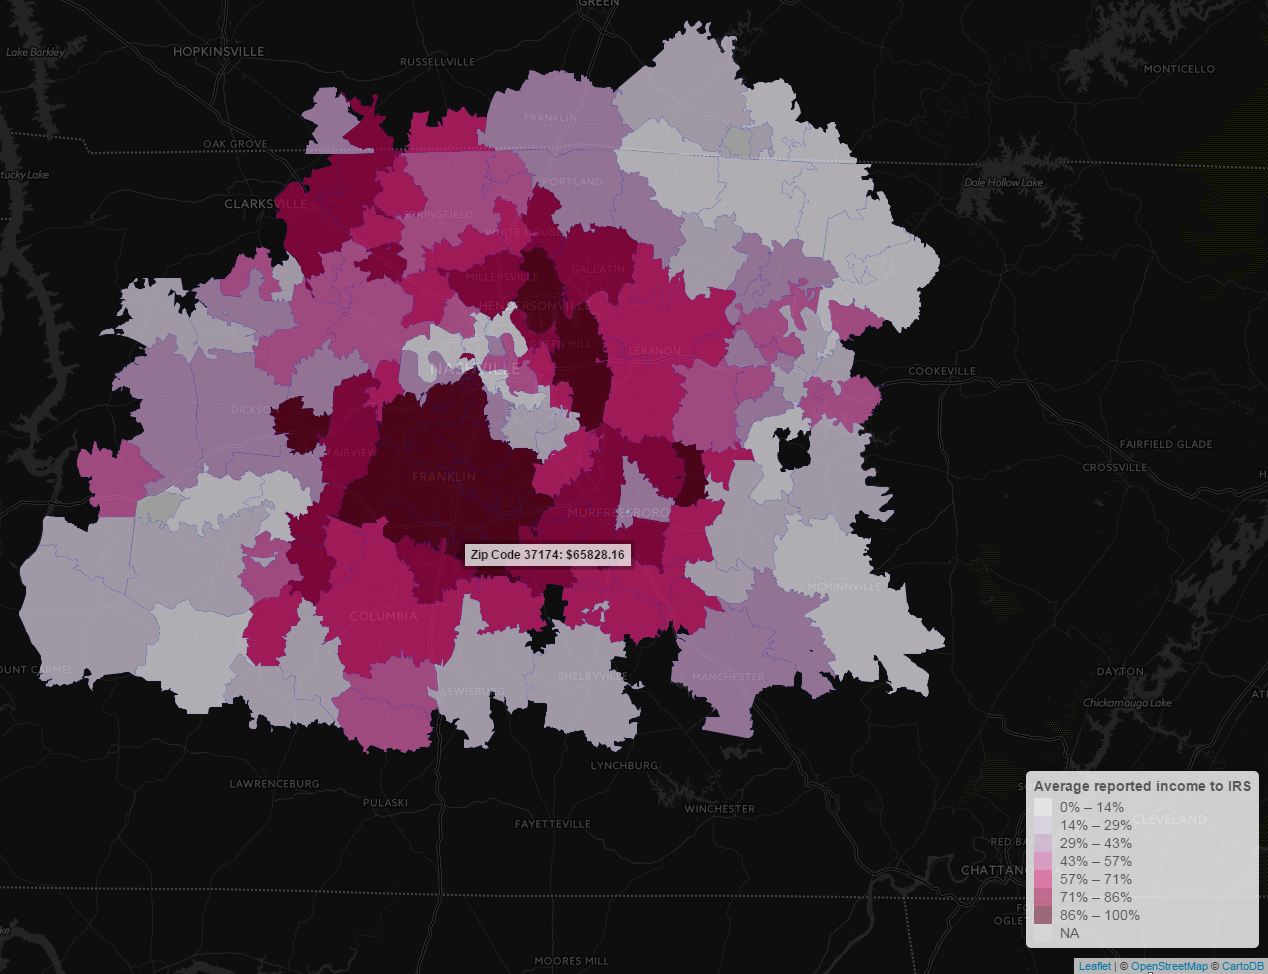
\includegraphics[width=\textwidth]{nashville}
  \caption{Interactive Leaflet map of average reported IRS income by zip code, Nashville, Tennessee area.}
  \label{figure:nashville}
\end{figure}

\begin{Schunk}
\begin{Sinput}
get_zips('Sacramento') %>% map_zips(palette = 'YlGnBu')
\end{Sinput}
\end{Schunk}

\begin{figure}[htbp]
  \centering
  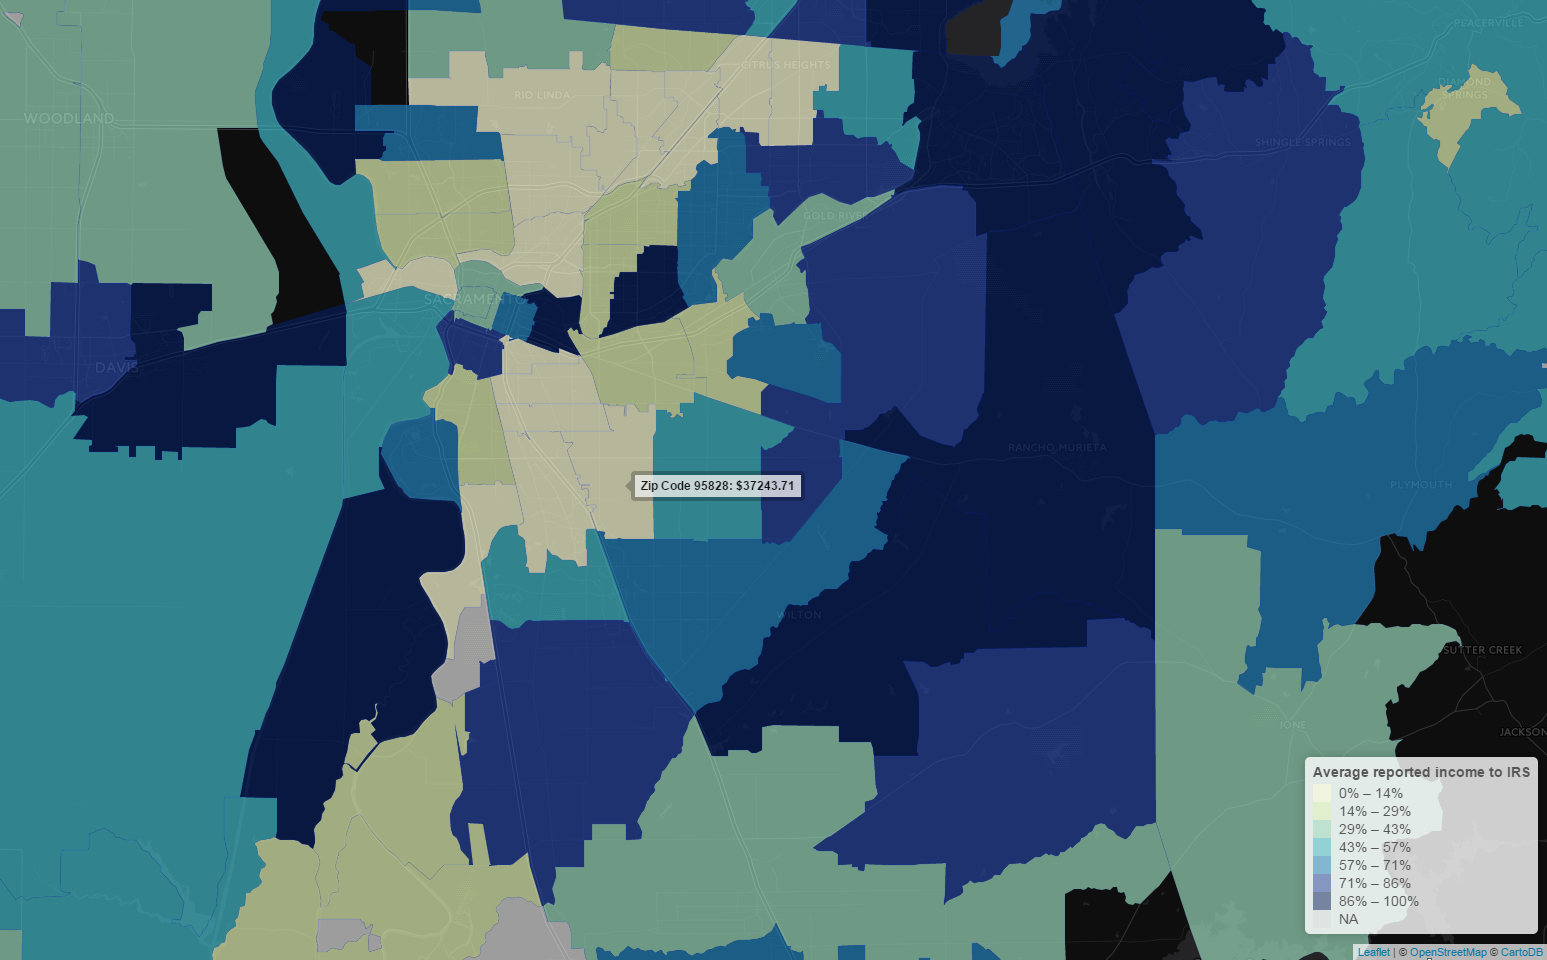
\includegraphics[width=\textwidth]{sacramento}
  \caption{Interactive Leaflet map of average reported IRS income by zip code, Sacramento, California area.}
  \label{figure:sacramento}
\end{figure}

\subsection{Conclusion}\label{conclusion}

Some comments here about how tigris fits in with other geospatial
analysis and visualization packages; how the R ecosystem rivals
traditional desktop GIS in its functionality and in many ways is more
flexible.

\bibliography{RJreferences}

\address{%
Kyle Walker\\
Texas Christian University\\
2850 S University Dr\\ Fort Worth, TX 76109\\
}
\href{mailto:kyle.walker@tcu.edu}{\nolinkurl{kyle.walker@tcu.edu}}

\address{%
Bob Rudis\\
\\
\\ \\
}


